% Template for ICASSP-2010 paper; to be used with:
%          mlspconf.sty  - ICASSP/ICIP LaTeX style file adapted for MLSP, and
%          IEEEbib.bst - IEEE bibliography style file.
% --------------------------------------------------------------------------
\documentclass{article}
\usepackage{amsmath,graphicx,02456}
\usepackage[utf8]{inputenc}    
\usepackage{enumitem}

\toappear{02456 Deep learning, DTU Compute}


% Example definitions.
% --------------------
\def\x{{\mathbf x}}
\def\L{{\cal L}}

% Title.
% ------
\title{Deep Reinforcement Learning for VizDoom}
%
% Single address.
% ---------------
\name{Martin Simon* (S163008), Niels Justesen$\dagger$ (S165591), Søren Jesper Bloch* (S123809)}
\address{* Technical University of Denmark,  $\dagger$ IT University of Copenhagen}

%
% For example:
% ------------
%\address{School\\
%	Department\\
%	Address}
%
% Two addresses (uncomment and modify for two-address case).
% ----------------------------------------------------------
%\twoauthors
%  {A. Author-one, B. Author-two\sthanks{Thanks to XYZ agency for funding.}}
%	{School A-B\\
%	Department A-B\\
%	Address A-B}
%  {C. Author-three, D. Author-four\sthanks{The fourth author performed the work
%	while at ...}}
%	{School C-D\\
%	Department C-D\\
%	Address C-D}
%
\begin{document}
%\ninept
%

\maketitle
%
\begin{abstract}
(Martin)
As Deep Reinforcement Networks have progressed fast, autonomous agents have started to outperform humans in simple games such as the ones made by Atari in the 80s. In our coursework we combined monochrome pixel data with game feature information to train a Deep Q Network to play Doom in its Artificial Intelligence Research Platform: ViZDoom. By training the policy in separate learning phases, first with a navigation reward and then with a shooting reward, the policy succeeded to show significant improvement in only 2x200 epoch leaning. The policy developed a very specific strategy and scored higher than average built-in bots. The strategy was especially successful in the ViZDoom death match scenario.

\end{abstract}
%
\begin{keywords}
neural networks, deep reinforcement learning, Q-Learning, first-person perspective games, policy gradient method, reward shaping, Deep Q Networks
\end{keywords}

\section{Introduction (Søren)}
\label{sec:intro}
The goal of this project is to teach an AI how to play the ZDoom using deep reinforcement learning (an open source version of Doom 2 (a 3D shooter from 1995) that contains parts of the original source code) using nothing but the visual output and scoring variables using ViZDoom to determine the action to take.
ViZDoom, an open source environment meant for creating and teaching an AI to play ZDoom, is utilized to help achieve this goal. In this report we will go through the various methods and variables and what result they yielded or is likely to yield.
Deep learning has had a lot of success in other older games such as the old Atari games\cite{mnih2015human} and is in most cases better than linear learning, in a great number of cases the AI policy even reaches beyond human levels in terms of ability \cite{silver2016mastering}. In this project we aimed to create an AI policy that goes beyond that of the default build in AI, in this we where successful although one may argue that is just because the policy prefer bigger weapons over smaller ones because of their ammo consumption. The project source code can be found here\footnote{https://github.com/njustesen/vizdoom-ai}.
% Commecnts by Niels:
% Our goal is to learn a policy using deep reinforcement learning. AI is a bit to vague.
% Very short. You could add an intro on what other people achieved with deep reinforcement learning. Cite the DeepMind Atari paper (see references). Have other people done this? Mention and cite the compeition and other ViZDoom papers (see references).
% Mention what our exact goal is and whether it was reached.



\section{Deep Reinforcement Learning}
\label{sec:format}

\subsection{Markov Decision Processes (Niels)}
This section will go through some of the theory on deep reinforcement learning that was used in our experiments. In reinforcement learning the goal is to find an optimal policy for a Markov Decision Process (MDP). A MDP consists of a set of possible states $S$, a set of available actions $A$, a probabilistic state transitioning function $P_{a}(s,s')$ determining the probability of transitioning from $s$ to $s'$ by taking action $a$. Finally an MDP also has a reward function $R(s,s')$ that determines the reward of transiting to states. The problem in MDPs is to find an optimal policy $\pi$ that maximizes the expected future reward. The expected future reward when being in state $s$ using policy $\pi$ can be described using the Bellman equation:

\begin{equation}
V^\pi(s)= R(s,\pi(s)) + \gamma \sum_{s'} P(s'|s,\pi(s)) V^\pi(s') 
\end{equation} 

where $\gamma \in [0:1]$ is a discount factor that gives rewards in the near future higher value than rewards in the far future. Two reinforcement learning methods were implemented in this project and will be described below using the terminology of MDPs and the Bellman equation.
 
\subsection{Deep Q Networks (Niels)}
Google's DeepMind has recently achieved human-level control in a range of Atari games using a deep reinforcement learning algorithm called Deep Q Networks (DQN) \cite{mnih2015human}. DQN implements the traditional Q-learning algorithm using a deep neural network such as a convolutional neural network (ConvNet). Such networks are able to learn complex policies from just raw pixel inputs. In Q-learning a Q-function $Q(s,a)$ is learned that estimates the discounted future reward by taking action $a$ in state $s$. A policy can then use the Q-function by taking the action that leads to the highest future reward $\max_{a}Q(s_{t}, a)$. 

Agents observe and act in discrete time intervals in MDPs. For each action made by an agent a so-called trajectory $<s_{t}, a. s_{t+1}, r_{t+1}>$ is obtained, where action $a$ taken in state $s_{t}$ results in state $s_{t+1}$ and a reward $r_{t+1}$. Using this trajectory the Q-function is incrementally updated using the Q-learning update rule, which is based on the Bellman equation. First the learned value $y$ is calculated from our trajectory:

\begin{equation}
y = r_{t+1} +\gamma \cdot \max_{a}Q(s_{t+1}, a)  
\end{equation}

Then the error $\delta$ is calculated which is the difference between the learned value $y$ and our current estimation of $Q(s_{t},a_{t})$.

\begin{equation}
\delta = y - Q(s_{t},a_{t})
\end{equation}

Finally $Q(s_{t},a_{t})$ is updated with $\delta$ using a learning rate $\alpha \in [0:1]$.

\begin{equation}
Q(s_{t},a_{t}) \leftarrow Q(s_{t},a_{t}) + \alpha \cdot \delta    
\end{equation}

In DQN the Q-function is a neural network and is updated using Stochastic Gradient Descent (SGD) with backpropagation. The error backpropagated is $\delta$ and SGD uses $\alpha$ as the learning rate.  

\subsection{Experience Replay (Niels)}

A key improvement to DQN is \emph{experience replay} \cite{mnih2015human}. The naive approach in DQN is simply to collect $n$ consecutive trajectories, where $n$ is the batch size, and backpropagate the error from this mini-batch. The issue with this approach is two-fold. The first issue is that it learns from very correlated trajectories that will produce very inaccurate updates and ultimately result in slow learning ending in local optimum. The second issue is that trajectories are only used for learning once and then deleted, while they just as well could be reused. 

\begin{figure}[htb]

\begin{minipage}[b]{1.0\linewidth}
  \centering
  \centerline{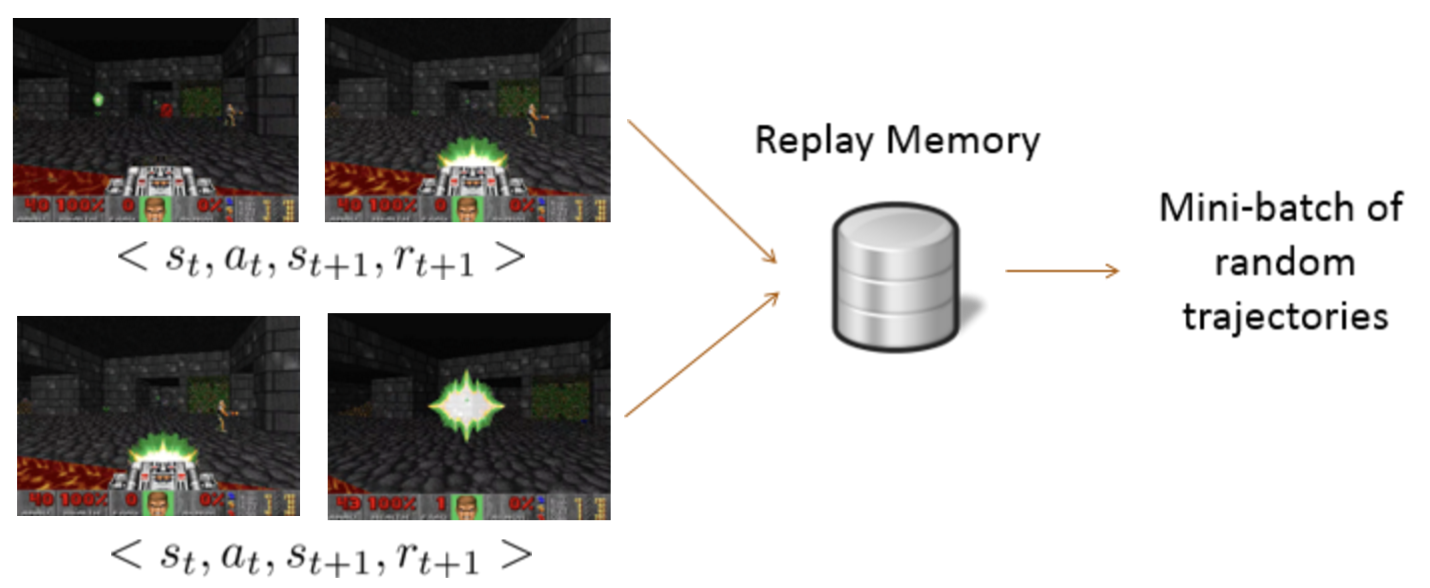
\includegraphics[width=8.5cm]{experience}}
%  \vspace{2.0cm}
\end{minipage}
\caption{Trajectories are added to a replay manager as the agent interacts with the environment. At some fixed interval a mini-batch of randomly selected trajectories are pulled.}
\label{fig:res2}
%
\end{figure}

The experience replay method solves these two issues by storing observed trajectories in a replay memory. The memory will have a fixed size and the oldest trajectories will be overridden when it is full. A mini-batch of trajectories are at some fixed interval randomly pulled from the replay memory and used by the SGD. 

\subsection{Deep Recurrent Q Networks (Niels)}

In some environments it is not possible to capture the entire state from a single time step. It is e.g. not possible to capture the speed and direction of moving objects from a single frame in a video game. A single frame in VizDoom also shows only a very limited part of the level and it is therefore often said that the Q-function estimates observation-action value $Q(o,a)$ instead of the state-action value $Q(s,a)$. For some environments it is necessary to use multiple consecutive observations as input to the DQN. This approach was also used by \cite{mnih2015human} where four frames were stacked as input to the network.

Another approach that was implemented in our project is the Deep Recurrent Q Network (DRQN) which has been shown to be superior to the stacking DQN approach \cite{hausknecht2015deep} in some games where observations only show the partial state. In DRQN a recurrent layer is added to the network just before the output layer to implement a many-to-many Recurrent Neural Network (RNN) architecture. DRQN was also used by \cite{lample2016playing} with Long Short-Term Memory (LSTM) cells to achieve good results in ViZDoom. 


\begin{figure}[htb]

\begin{minipage}[b]{1.0\linewidth}
  \centering
  \centerline{\includegraphics[width=6.0cm]{drqn}}
%  \vspace{2.0cm}
\end{minipage}
\caption{How the hidden state of the recurrent layer in DRQN is propagated through time following the many-to-many RNN architecture. In our model LSTM gates were used.}
\label{fig:res}
%
\end{figure}

Training of the DRQN can be done in several ways. We choose to focus on the approach by \cite{lample2016playing}. During training sequences of trajectories of length $n$ are sampled from the replay memory. The input shape thus becomes [$bath\_size$, $n$, $frame\_width$, $frame\_height$, $color\_channels$]. The trajectory sequences are then fed through the network, but only the last part of the outputs are used for backpropagation while the first part is used only to initialize the hidden state. The first part is called \emph{observation history}. After the policy is trained the hidden state of the network is stored after each activation of the network and is feed as an additional input for the following activation. 

\subsection{Policy Gradient (Martin)}

Instead of using value functions to optimise the loss function the Policy Gradient Method was also implemented. This method uses real-time gained experience by evaluating the policy gradient change direction to make available action decisions.

\section{Approach}
\label{sec:pagestyle}

\subsection{Models (Martin)}

The monochrome 48x64 pixel data was imported to the first layer (see Figure 3). Two convolutional layers with respectively 32 and 64 filters were used for training with this input data. The output was projected to a fully connected layer and then translated to four actions (move left, right, forward and shoot).
\begin{figure*}[!htb]
  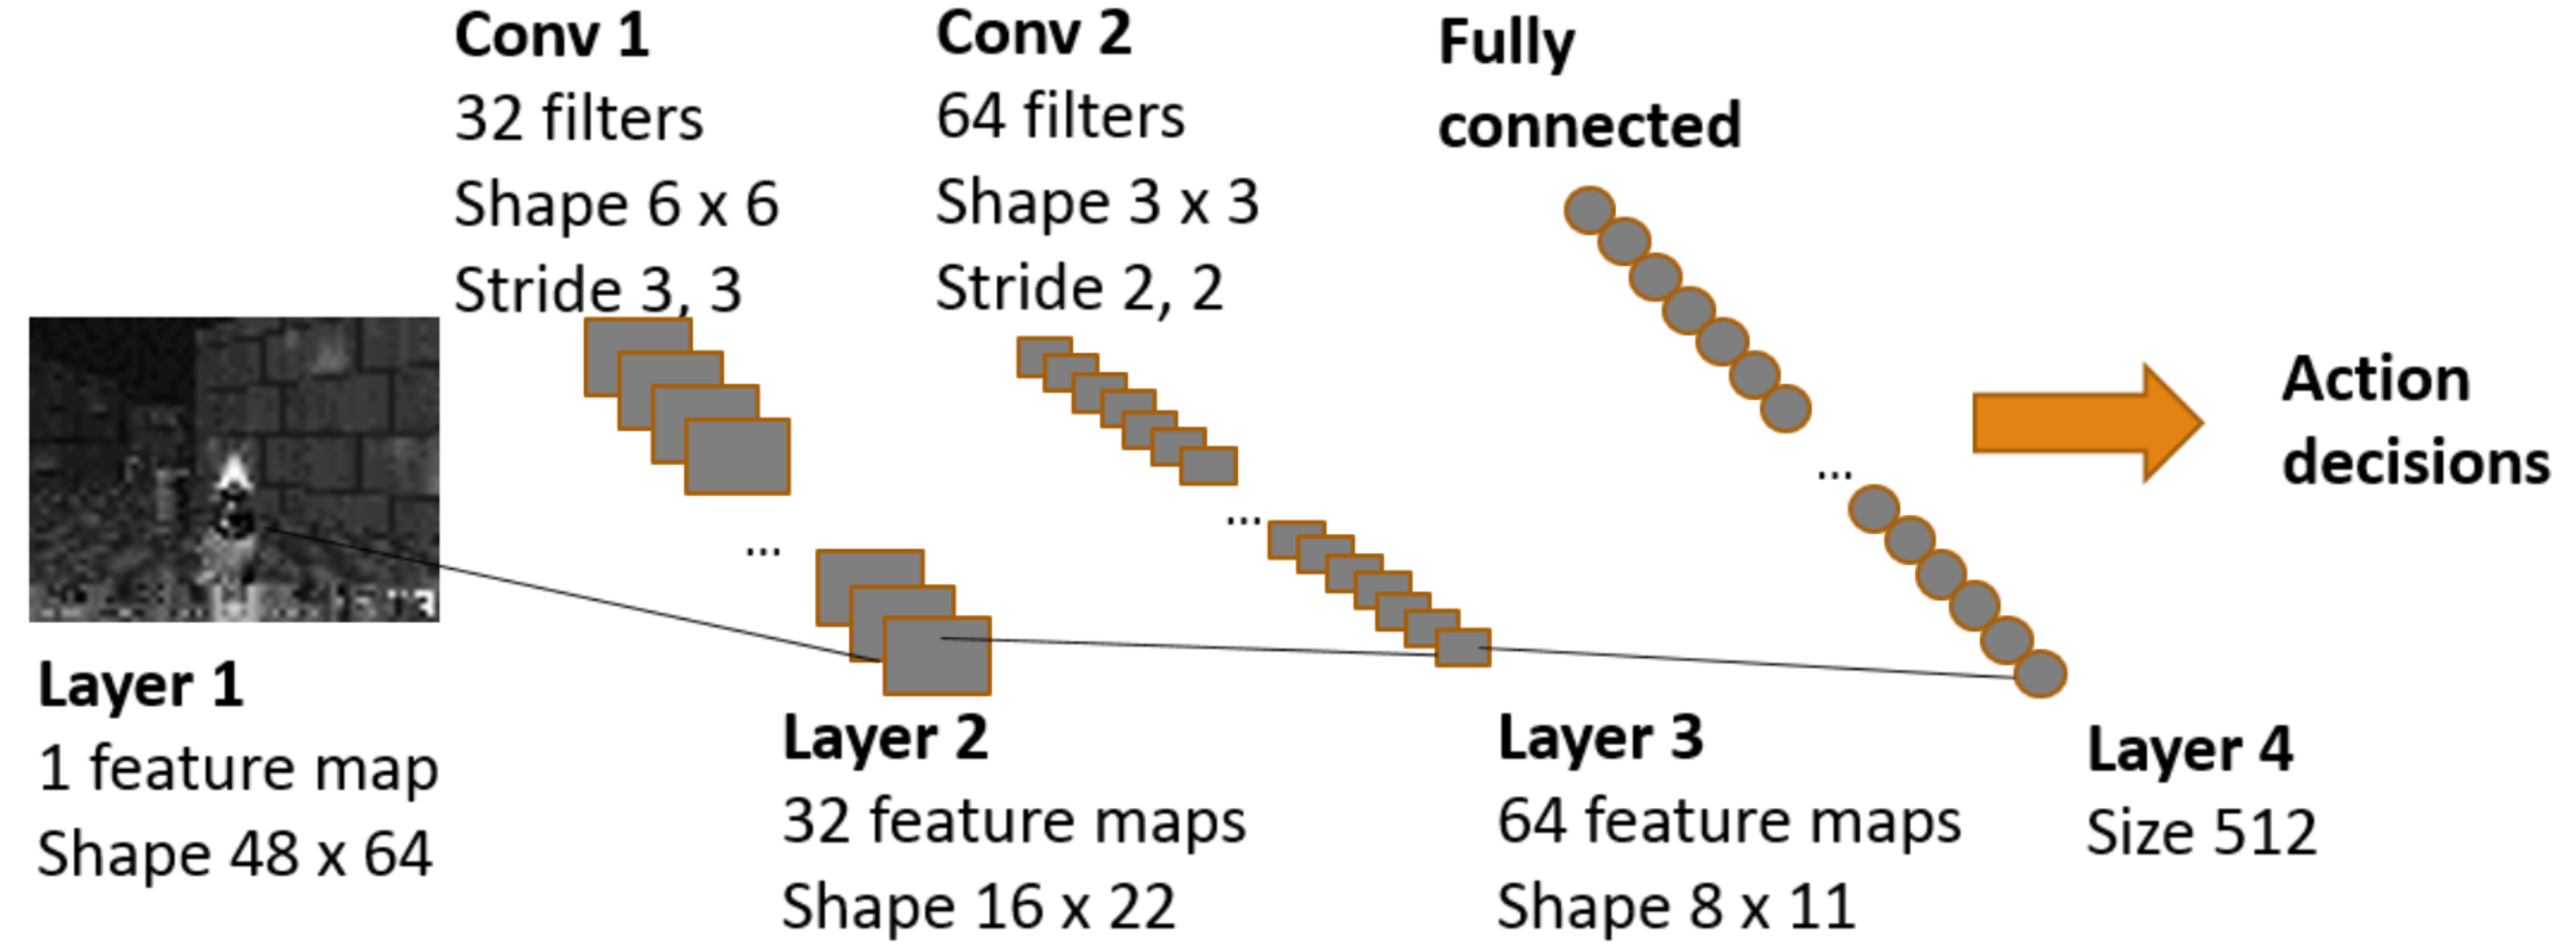
\includegraphics[width=0.8\textwidth]{model}
  \centering
  \caption{Illustration of DQN Model layout. 
  }
\end{figure*} 

The DRQN model used in the experiments were identical to the DQN model but with on additional layer added. A layer of 512 LSTM cells were added after the fully connected layer. The number of cells were picked to be identical to the size of the previous layer. 

\subsection{Root Mean Squared Gradient \& RMSprop (Martin)}
In optimization functions RMSProp with size 64 mini batches was used for gradient calculations. It is largely recommended as a basic method for learning methods in a large neural network with a large redundant data set. RMSProp is a method of using the sign of the gradient combined with the root of the nearby averaged square gradients to decide on the step size. This makes it more usable for mini-batches unlike RProp, which uses only the sign of the gradient. 
Although Google DeepMind improved the factors in the regular gradient, there was mild improvement compared to the regular RMSProp when applied to a similar Q-Learning tasks and only showed better performance after millions of epochs as it continued to learn \cite{kurekdeep} \footnote{http://maciejjaskowski.github.io/2016/03/09/space-invaders.html}. 



\subsection{Divide and Conquer (Søren)}
In order to create a fully functional AI, the AI will need to try a lot of different combinations for different actions, and these actions may not be related to one another, which means that the complexity of the learning process can be reduced by splitting the process into smaller more direct tasks. By dividing up each of the task that is sought to be accomplished, and then conquering each of them individually, a result may be reached faster than without. In our case we utilized this by teaching it to walk and explore and shoot separately. By teaching it to walk first, we were able to have it reach scenarios were is possible to shoot the enemies, therefore it does not need to guess the walking procedure and can focus on learning where to aim and when to pull the trigger.

More specifically, we first trained the policy with one reward function using the $\epsilon$-greedy strategy with $\epsilon$ going from 100\% to 10\%. After this first phase of training the learned policy (or network parameters) was trained further with a new reward function and $\epsilon$ going from 50\% to 10\%, thus utilizing what was learned in the first phase during training in the second phase.

% Comments by Niels:
% Continue by how we did this specifically:
% First we trained the policy 200 epochs with one reward function using epsilon-greedy 100% -> 10%. Then we used another reward functon with epsilon-greedy 50% -> 10%.

\subsection{Navigation Reward (Niels)}
\label{sec:navigation}
A reward function was implemented to make the agent navigate the level in the deathmatch scenario. To access the players position we had to change the ViZDoom source code and recompile it. The naive approach to train an agent to navigate would be to give a reward when the game ends relative to the total distance travelled by the agent. This has two issues; (1) it creates very sparse rewards that will be difficult learn and (2) walking in circles is just as good as exploring all the different areas in the level. Our approach gives a reward at every time step in the game and solves these two issues. It uses the following formula to calculate the reward:

\begin{equation}
R(s_{t}, s_{t+1}) = \sum_{\tau = 0}^{t+1} \beta^{t+1-\tau} \big(|p(s_{t+1}) - p(s_{\tau})| - |p(s_{t}) - p(s_{\tau})|\big)
\end{equation}

where $p(s)$ is the position of the player in state $s$ and $\beta \in [0:1]$ is a constant that determines to what degree movement away from recent positions are rewarded higher than movement away from past positions. This reward function rewards movement away from previous positions by comparing the distance to all previous positions at $t+1$ by the distance to all previous positions at time $t$. Several experiments were attempted to come up with this solution. 

\subsection{Shooting Reward (Martin)}
As the implementation of the model trained with exploration reward increases the probability of finding bots, a function was applied to reward decrease of ammo when enemies were detected. 
\begin{equation}
R(s_{t}, s_{t+1}) = \big|a(s_{t}) - a(s_{t+1})| \cdot e(s_{t+1}\big)
\end{equation}
where $a(s)$ is the amount of ammo available for the player in state $s$ and $e(s)$ the amount of enemies in range. 

\subsection{Damage Reward (Søren)}
Since the damage necessary to kill an opposing player is not necessarily meet with the weapon equipped, the AI will not necessarily learn how to kill enemy players. however if it is rewarded for damaging enemy players, it is more likely to approach a solution were it will kill the enemy player. In order to accomplish this we had to modify the very core of ViZDoom, as it does not normally give this output, so the memory buffer which returns the desired variables to us had to be altered to contain this info, and we had to find one of the areas were damage is given, which we found but it is utilized by everything, causing the code to currently have issues with environmental damage, causing an unhandled exception, we mainly see this when the player tries to go through lava. Our changes to ViZDoom can be found on GitHub\footnote{https://github.com/neroes/ViZDoom}.

% Comments by Niels:
% Fix typos.
% Write that we needed to change the ViZDoom source code. What did you exactly try and what worked?

\section{Results}


% Comments by Niels:
% TODO: Anyone?

\subsection{System Specifications (Søren)}
\label{sec:systems}
In order to test these ideas we used 2 different setups, system 1 was a machine to which Niels was granted access in order to run these simulations from ITU, and system 2 was a private machine built by Martin.
\begin{center}
  \begin{tabular}{ | l | c | r | }
    \hline
      & Test System 1 \\ \hline
    CPU & Intel(R) Core(TM) i7-5820K CPU   \\ \hline 
    GPU & 2 x GeForce GTX TITAN X \\ \hline
    RAM & 32GB 2666MHz DDR4 Ram \\ \hline
  \end{tabular}
\end{center}



\begin{center}
  \begin{tabular}{ | l | c | r | }
    \hline
      & Test System 2 \\ \hline
    CPU & Intel(R) Core(TM) i7-3720QM CPU  \\ \hline 
    GPU & GeForce GTX 750 Ti \\ \hline
    RAM & 24GB 1600Mhz DDR3\\ \hline
  \end{tabular}
\end{center}

% Comments by Martin - I added my data, but haven't yet figured out how to put the table in line. Maybe thi is ok configuration?

\subsection{Basic Scenario (Niels)}
\label{sec:basic_scenario}
Our first experiments were made on the basic ViZDoom scenario where the the agent is located in a room with one enemy. If the enemy is hit it is killed and the agent is rewarded with 100 points. For every bullet used the agent is given a negative reward of -5. Our DQN model was able to learn an almost perfect policy for this problem within 30 minutes on Test System 1 using the CPU (see Figure \ref{fig:basic-dqn}). The configurations used were the following:

\begin{itemize}[noitemsep]
\item Replay memory size = 100,000
\item Frame skip = 4
\item Update frequency = 4
\item Learning steps per epoch = 2000
\item Batch size = 64
\item Learning rate = 0.00025
\item Discount factor = 0.99
\end{itemize}

\begin{figure}[htb]

\begin{minipage}[b]{1.0\linewidth}
  \centering
  \centerline{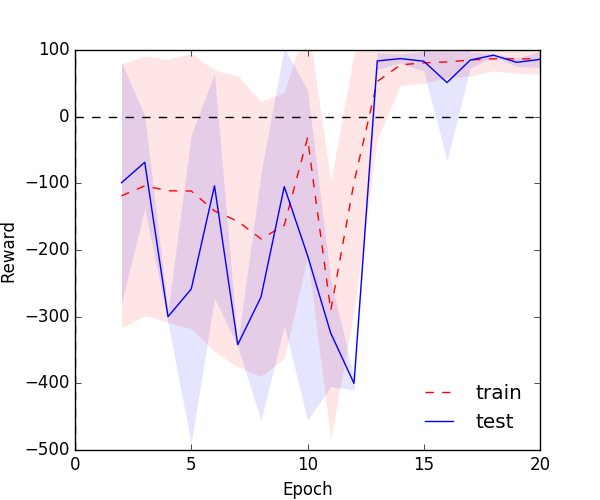
\includegraphics[width=8.5cm]{basic_adv}}
%  \vspace{2.0cm}
\end{minipage}
\caption{Rewards per. episode in the basic scenario with DQN. Opaque fill shows standard deviation. }
\label{fig:basic-dqn}
%
\end{figure}

The policy gradient method was also tested in this problem several times but always ended in a local optimum such as shooting without moving. Several experiments were made with different hyper-parameters such as the following:

\begin{itemize}[noitemsep]
\item Frame skip = 4
\item Learning rate = 0.1
\item Discount factor = 0.99
\end{itemize}

The DRQN model was also tested in this problem without success. We expected that it would take much longer to train, but 3 hours of training on Test System 1 with GPU showed no sign of progress at all. It is unclear to us why it failed to learn. The configurations were the same as for the DQN but with the following additions:

\begin{itemize}[noitemsep]
\item Observation history = 4
\item History = 10
\end{itemize}

Based on these results from the basic scenario we decided to focus only on DQN. We expect that with more debugging and testing the DRQN model should work just as well as the DQN model for this problem. 

\subsection{Deathmatch Navigation (Niels)}
The DQN model was tested in the deathmatch scenario without enemy bots using the navigation reward (see Section \ref{sec:navigation}). The same configuration as in Section \ref{sec:basic_scenario} were used. For the navigation reward function the $\beta$ constant was set to 0.95. The training ran on for $\sim$8 hours on Test System 1 and achieved a satisfying result. The trained policy was able to navigate through more than half of the level in a very human-like manner with some distinct issues. Sometimes, but rarely, it can get stuck by continuously walking into an explosive barrel. Another issue is a corner in the level where there is a mirror and the agent has some difficulties moving away from it. An example of the navigation policy can be seen on YouTube\footnote{https://www.youtube.com/watch?v=aSoToirhlhc}.

\begin{figure}[htb]

\begin{minipage}[b]{1.0\linewidth}
  \centering
  \centerline{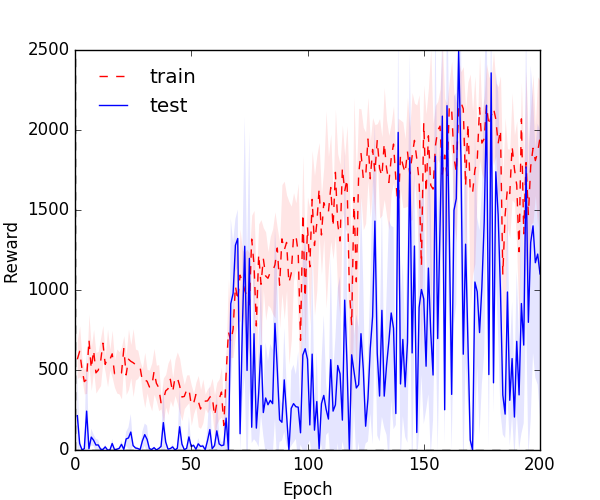
\includegraphics[width=8.5cm]{exploration}}
%  \vspace{2.0cm}
\end{minipage}
\caption{Exploration rewards per. episode obtained by DQN in the death match scenario. Opaque fill shows standard deviation.}
\label{fig:res}
%
\end{figure}

\subsection{Deathmatch Shooting (Martin)}
The trained policy swiftly learned to move in the center of a room full of enemies to shoot with its most ammo-consuming weapon. This way it managed to spend a large amount of ammo while in presence of many opponents. While the trained policy continued to get stuck sometimes, as exploration was not further improved in this training model, the improved model was now competitive with built-in bots by reaching approximately four kills per death during training. Although this kamikaze-style strategy would not be competitive against human players, it is a clear sign of progress when taken into account only 2x200 epochs of training.

\begin{figure}[htb]

\begin{minipage}[b]{1.0\linewidth}
  \centering
  \centerline{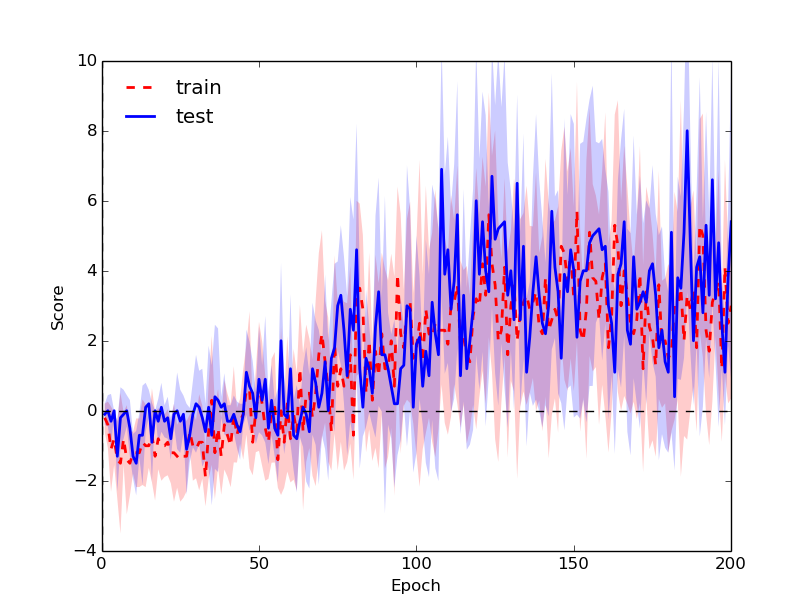
\includegraphics[width=8.5cm]{shooting_plot_2}}
%  \vspace{2.0cm}
\end{minipage}
\caption{Score of kills per death during Deathmatch Shooting training.
}
\label{fig:basic-dqn}
%
\end{figure}

The learned policy can be seen in this YouTube video\footnote{https://www.youtube.com/watch?v=oGt34SxL9h8}.

%\begin{figure}[htb]

%\begin{minipage}[b]{1.0\linewidth}
%  \centering
%  \centerline{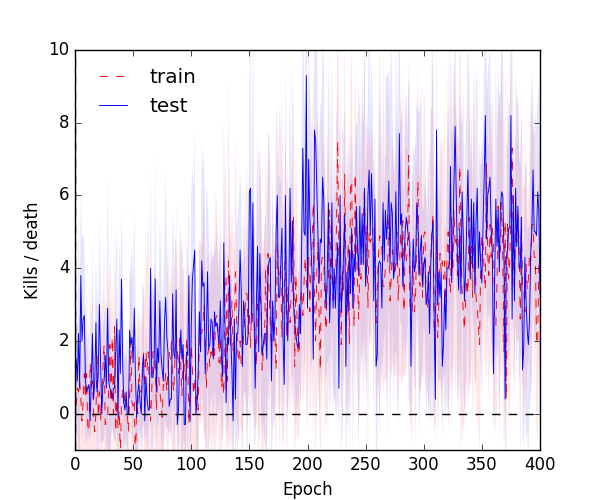
\includegraphics[width=8.5cm]{plot_dm_kill_400}}
%  \vspace{2.0cm}
%\end{minipage}
%\caption{Example of placing a figure with experimental results.}
%\label{fig:res}
%
%\end{figure}

\subsection{Final Evaluation (Martin)}
During final evaluation the trained model was set against seven built-in bots for 100 2-minute long games. As a result it averaged 3.4 kills per death and ranking on third place in the Hall of Fame.

\begin{figure}[htb]

\begin{minipage}[b]{1.0\linewidth}
  \centering
  \centerline{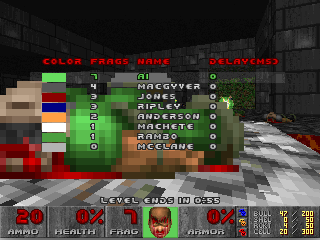
\includegraphics[width=8.5cm]{result}}
%  \vspace{2.0cm}
\end{minipage}
\caption{Example end-game screen where our agent won against the build-in bots.}
\label{fig:res}
%
\end{figure}
\newpage
\section{Discussion (Søren)}
While a perfect result where the machine learned the full relationship between killing an enemy and winning has not been found, we have however manage to get a kill/death ratio well above over 1\footnote{kill/death ratio shows the relationship between a players kills and death, meaning that if it is above 1, they player generally kills more than he dies and assuming that each opponent is of the same strength the player is better than average}. Meaning that our player is stronger than the average build-in bot, although it's caused by the player trying to shoot as many bullets as possible with as many as possible enemies on screen as possible, causing it to pick the weapon with the largest bullet consumption, these weapons have a large area of effect.
The Damage reward would likely yield more direct and more efficient especially in cases of non splash damage weapons, as we currently just shoot in their general direct not caring about the placement of the enemy on screen, we just care that they are there. Additionally the AI policy may be improved by various other measures, such as making it play against an earlier AI policy to train it further, in order to make it more capable at surviving and scoring against harder opponents. Although this would still not teach the AI policy to shoot its enemies rather than just shooting big weapons in their general direction, unless it gets a metric for damaging. Because we have so many ways of evaluating how well the AI policy has faired, we can most likely save on training time by going thought the various ways of scoring and then using the previous as the next ones starting, for instance we could start with the shooting reward, which makes us shoot in the right direction, then move onto damaging which would teach us to damage the enemy and finally move onto killing the enemy which is what we ultimately want the AI policy to do. 

\section{Conclusion (Martin)}
During this project we successfully trained a policy to outperform built-in bots of a first-person shooter game Doom by implementing the Deep Q Network (DQN) algorithm. Experiments with the Deep Recurrent Q Network architecture as well as the Policy Gradient method did however not show any positive results.

Two strategies for DQN were implemented. First a naive end-to-end training and then a divide-and-conquer strategy. Experimenting with a naive end-to-end training failed and the failure can be attributed to killing a bot being an extremely random event. Using the divide and conquer strategy the policy was first trained to explore the level and thereafter rewarded for ammo decrease while enemies were on the screen. Despite training for a limited amount of epochs due to lack of computational resources, the algorithm developed a clear winning strategy. This illustrates the necessity of having a clear understanding of the task handed to a network. 

Further improvements can be made by (1) increasing the number of epochs and (2) train the network against itself and (3) reward the agent when it deals damage to opponents.

\vfill
%\pagebreak

\bibliographystyle{IEEEbib}
\bibliography{refs}

\end{document}